\chapter{Validation der Kriterien am Beispiel Æthershards}
\label{cha:evaluation}

In diesem Kapitel wird ein Beispiel für die Spielidee eines location-based Games, im folgenden Æthershards genannt, gegeben. Die Spielidee wird mittels einer statistischen Erhebung überprüft. Aus Erkenntnissen, die sich aus der Erhebung ableiten lassen, wird die Spielidee überarbeitet. Die daraus entstandene Spielidee wird durch die in dieser Arbeit entwickelte Evaluation ausgewertet.

%Æthershards ist als ein neues virtuelles Haustier erdacht worden, das sich durch eine Hintergrundgeschichte und den Location-based Game Ansatz von anderen Videospielen unterscheidet. 


\section{Spielidee Æthershards}
Æthershards ist als ein neues virtuelles Haustier erdacht worden, das sich durch eine Hintergrundgeschichte und den Location-based Game Ansatz von anderen Videospielen unterscheidet. \\
In diesem location-based Game übernimmt der Spieler die Verantwortung für virtuelle Haustiere. Diese Tiere kann er in der realen Welt mittels Smartphone einfangen. Die gefangenen Tiere müssen regelmäßig versorgt werden. Der Spieler hat so die Aufgabe die Tiere zu füttern und zu unterhalten, damit sie nicht verhungern und sich wohl fühlen.\\ 
Anhand einer in Episoden unterteilten Geschichte sollen die Spieler einen zusätzlichen Anreiz haben ein Abenteuer mit ihren Tieren zu erleben. Durch die Unterteilung in Episoden lässt sich nach und nach eine umfangreiche Hintergrundgeschichte entwickeln, die beliebig erweitert werden kann. \\
Das fertige Spiel soll kommerziell Vermarktet werden. Aus diesem Grund sollte es plattformunabhängig sein. Eine Plattformunabhängigkeit ist in der Regel mit einem größeren Programmieraufwand verbunden. Daher kann es ggf. sinnvoll sein das Spiel vorerst nur für eine oder zwei Plattformen zu entwickeln. \\
Für das Spiel bieten sich drei verschiedene Einnahmequellen an. Die drei Möglichkeiten sind ein Festpreis, Werbeeinblendungen und Micropayments. Für Æthershards sind Werbeeinblendungen und Micropayments als Ertragsmöglichkeiten in Erwägung gezogen worden, da ein Festpreis als eine zu große Einstiegshürde angesehen worden ist. Durch Micropayments sollen die Spieler im späteren Spiel die Möglichkeit haben Gegenstände zu erwerben, die das Spiel kosmetisch verändern. Diese Gegenstände haben keinen spielerischen Vorteil, sie beeinflussen nur die Ästhetik des Spiels. Micropayments sind in diesem Zusammenhang als kleine Bezahlungen für virtuelle Gegenstände und Personalisierungen im Spiel zu verstehen.



%\chapter{Umgestaltung des Spielkonzepts}
%\label{cha:umgestaltung_spielkonzept}
%Dieses Kapitel beschreibt die zu Grunde liegende Spielidee. Der Augenmerk liegt auf der Evolution der Spielmechanik, da sich basierend auf dem Ergebnis der Erhebung an der ursprünglichen Konzeption Fehleinschätzungen gezeigt haben.


%\section{Ursprüngliche Konzeption}
%\label{sec:}
%An dieser Stelle muss vorab gesagt werden, dass das Spiel anfangs als virtuelles Haustier geplant worden ist, die grundlegende Spielidee sich aber mit dem wachsenden Wissensstand mehr und mehr transformiert hat.
 
%Diese Skizze ist eine der ersten von uns erstellten Skizzen zur Spielmechanik. Sie soll zeigen welche Features ursprünglich geplant wurden. Im Folgenden werden einzelne Punkte der Zeichnung erläutert um deren Sinn und Zweck zu klären.



%\section{Wahl des Anbieters} 
%\label{sec:}
%Evtl. auslassen\\
%Großer Zeitaufwand\\
%Viele Anbieter sind nicht kostenlos.

\section{Statistische Erhebung zum Spiel Æthershards}
%Einzelne Fragestellungen und Ergebnisse im Detail} 
%\label{sec:}
Vor der weiteren Konzeptionierung des Spiels wurde eine Umfrage erstellt, um die Qualität der Spielidee Æthershards zu überprüfen. Dies ist notwendig, da eine Spielidee mit minderer Qualität automatisch zu einer schlechteren User Experience führt. \\
Ziel dieser Erhebung ist es durch gezielte geschlossene Fragen den Hintergrund der einzelnen Personen grob zu kategorisieren und ihren Geschmack bezüglich Videospielen zu skizzieren. Anhand dieser Umfrage soll festgestellt werden welche Ideen weiter verfolgt und welche wieder verworfen werden sollen. Besonders wichtig sind hierbei die folgenden Unterpunkte:
\begin{itemize}
\item Die Frage, ob sich die Spieler in Spielen eine Hintergrundgeschichte wünschen.
\item Die Frage, ob überhaupt der Wunsch besteht zum Spielen nach draußen zu gehen, um an einem location-based Game teilnehmen zu können.
\item Die Frage, ob und in wie weit die Spieler gewillt sind Werbeeinblendungen anzuschauen oder das Spiel durch Micropayments zu finanzieren.
\end{itemize}
Für einen Einblick in die Wünsche der Spieler werden zusätzlich offene Fragen zur Kritik an virtuellen Haustieren gestellt. \\
An der Umfrage konnte in einem Zeitraum von 14 Tagen teilgenommen werden. Sie war anonym und wurde online durchgeführt. Dieses Angebot wurde von 87 Personen wahrgenommen. \\
Im Folgenden werden die einzelnen Fragen der Umfrage genauer betrachtet und in Beziehung zueinander gesetzt.



\begin{description}
\item[Alter und Freizeitverhalten] 
%\label{sec:}
Zunächst wird das Alter (Abbildung \ref{chart:alter}) und die Freizeitbeschäftigungen (Abbildung \ref{chart:freizeit}) betrachtet. Es soll überprüft werden, ob es Auswirkungen vom Alter auf das Freizeitverhalten gibt. Beim Alter wurden die Altersbereiche über 16 Jahre bis 28 Jahre kategorisiert \cite{Statista:TXdt3fYx}. 
Die Freizeitbeschäftigungen sind grob in drei Kategorien eingeteilt. Die erste und am meisten gewählte Kategorie beinhaltet alle Aktivitäten, die in Verbindung mit Bildschirmen stehen, wie Computerspiele spielen und Fernsehen schauen. In der nächsten Kategorie befinden sich Aktivitäten die im Freien stattfinden. Die dritte Kategorie umfasst zwei Punkte der Umfrage, die den Titel nicht nutzbare Freizeit tragen kann. Dazu gehört zum einen das auf Grund der Beschäftigung keine Zeit für Freizeit bleibt oder das auf Grund fehlender Motivation keiner Freizeitbeschäftigung nachgegangen wird. 

\begin{figure}[H]
    \centering
    %trim=left buttom right top
    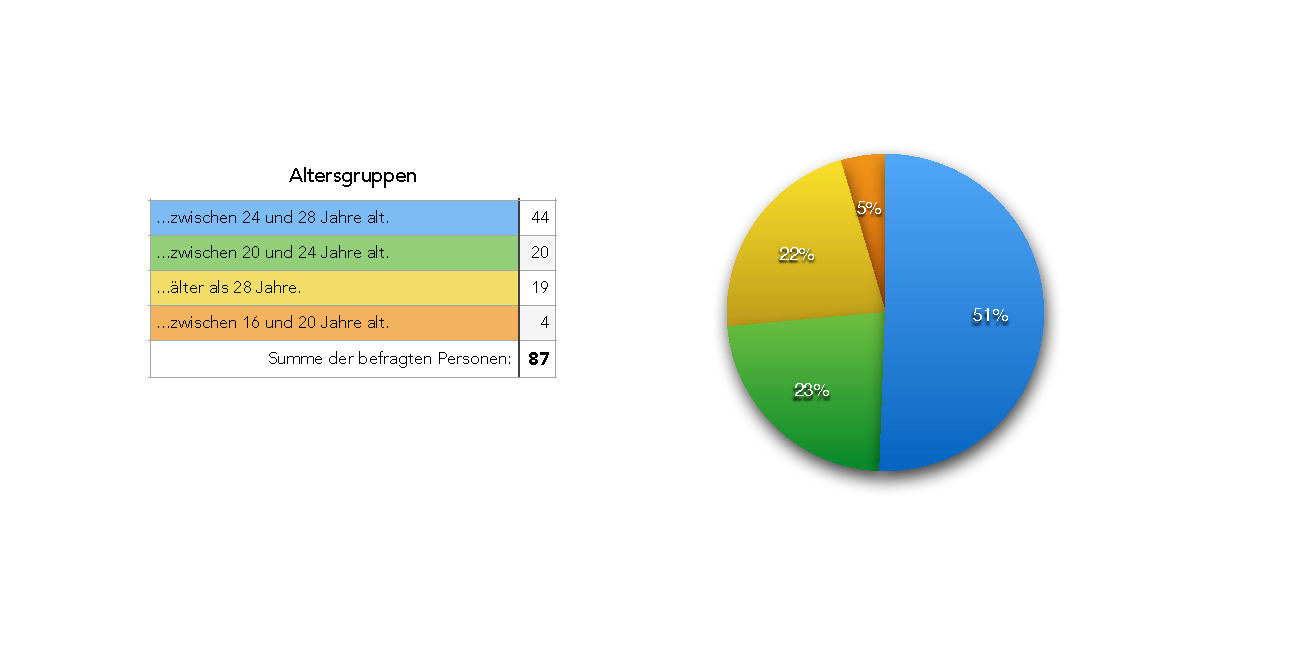
\includegraphics[trim=40 75 30 70,clip,width=1.2\textwidth, page=1]{files/statistik/umfrage1Ergebnisse.pdf}
    \caption{Altersverteilung der befragten Personen}
    \label{chart:alter}
\end{figure}
\begin{figure}[H]
    \centering
    %trim=left buttom right top
    \includegraphics[trim=40 75 30 70,clip,width=1.2\textwidth, page=2]{files/statistik/umfrage1Ergebnisse.pdf}
    \caption{Freizeitverhalten der befragten Personen}
    \label{chart:freizeit}
\end{figure}



%Obwohl beide Diagramme (Abbildung \ref{chart:alter} \& \ref{chart:freizeit}) den Eindruck erwecken, als seien die Freizeitaktivitäten stark mit dem Alter der befragten Personen verknüpft, ist das nicht der Fall. 
%Obwohl alle Personen über 28 Jahren in einer Gruppe zusammengefasst wurden, war sie nicht überrepräsentativ vertreten.
%Nur zufällig sind genau 44 befragte Personen zwischen 24 und 28 Jahre alt und auch genau sechsundvierzig Befragte verbringen ihre Freizeit größtenteils vor Bildschirmen. 
In allen Altersgruppen sind Personen vorhanden, die in ihrer Freizeit Fernsehen, Videospiele spielen, im Internet surfen usw.. Es lässt sich folglich nicht vom Alter auf das Freizeitverhalten und umgekehrt schließen.\\
So sind die beiden Personen, die bei der Frage nach der Freizeit \glqq Langeweile\grqq\ angegeben haben zwischen 20 und 24 Jahren. Des Weiteren haben auch Personen im Alter von 20 Jahren auf Grund ihrer beruflichen Verpflichtungen wenig bis keine Freizeit.  \\
Das Ergebnis der Umfrage zeigt eine klare Vorliebe für Freizeitaktivitäten vor diversen Monitoren. Da das Spielkonzept von Æthershards darauf ausgelegt ist auf einem Smartphones spielfähig zu sein und Location-based Inhalte benutzt, werden gleichzeitig die beiden größten Gruppen der Abbildung \ref{chart:freizeit} angesprochen. Demzufolge sind dies 78\% der befragten Personen.



\item[Smartphone-Verteilung]
%\label{sec:}

Die Fragestellung zum Smartphone soll Aufschluss darüber geben, wie sinnvoll es ist das Spiel plattformübergreifend zu entwickeln. %Plattformübergreifende Software läuft auf mehreren Betriebssystemen. %Es ist für Æthershards geplant mindestens auf iOS (iPhone) und Android lauffähig zu sein. 
Diese beiden Betriebssysteme werden laut Abbildung \ref{chart:smartphoneverteilung} von 89\% der befragten Personen benutzt.

\begin{figure}[H]
    \centering
    %trim=left buttom right top
    \includegraphics[trim=40 75 30 70,clip,width=1.2\textwidth, page=3]{files/statistik/umfrage1Ergebnisse.pdf}
    \caption{Darstellung der Smartphoneverteilung}
    \label{chart:smartphoneverteilung}
\end{figure}


Nach einer öffentlichen Statistik sind die Erträge durch die Apps auf iOS Geräten wesentlich höher als bei Android Geräten. \glqq Im Klartext heißt das, wenn ein Entwickler mit einer iOS-App im App Store 1 Euro verdient, spielt die gleiche App für Android ... im Google Play Store nur 0,23 Euro [ein].\grqq\ \cite{Hesse:2012ws} Eine Vermarktung über den iOS-Appstore würde demnach zu mehr als dem vierfachen Ertrag führen. Es ist zu beachten, dass 70\% der Befragten ein Android Smartphone besitzen und nur 18\% ein iPhone. Trotzdem lässt sich mit einer iOS App ein höherer Gesamtertrag erzielen.

%Unabhängig vom Alter und der Präferenz des Smartphone-Betriebssystems 



%Die Verteilung in beiden Diagrammen (\textbf{Abbildung \ref{chart:smartphone}}) ist ähnlich. 
%Von den Befragten besitzen ca. 70\% ein Google Android, ca. 20\% ein iPhone von Apple und ca. 7\% ein Windows Phone. Im letzten Punkt unterscheiden sich beide Erhebungen minimal. In der öffentlichen Statistik wird an dieser Stelle das BlackBerry angeführt. In der Umfrage des Authors ist dieser Punkt größer abgesteckt. So fallen hierunter weitere Smartphones sowie das Nichtvorhandensein eines Smartphones. \\
%Da beide Auswertungen so nah bei einander liegen, kann davon ausgegangen werden, dass bei der vom Author gestellten Erhebung ein relevanter Querschnitt entstanden ist.\\


\item[Hintergrundgeschichte] 
%\label{sec:}
Für das Spiel Æthershards ist eine Hintergrundgeschichte vorgesehen.  Daher zielt eine Frage speziell auf die Komplexität der Storyline ab. In Abbildung \ref{chart:story} werden die zugehörigen Ergebnisse dargestellt. 
%In der Umfrage wird dies mit einer direkten Frage zur Komplexität der von Geschichten in Spielen aufgegriffen. 
Exakt 86\% der Befragten äußerten sich positiv auf die Frage nach einer Hintergrundgeschichte. 
%finden eine Hintergrundgeschichte umso besser, je detaillierter sie ist bzw. sehr gut. 
Weitere 11\% haben sich einschränkend positiv geäußert. Nur 2\% der Befragten sprechen sich gegen eine Story aus. \\
Das Ergebnis ist laut der Umfrage weder alters- noch betriebssystemabhängig. Von allen Altersgruppen und Smartphone-Besitzern wird eine Hintergrundgeschichte gewünscht. \\ 
Hieraus lässt sich erkennen, wie wichtig eine Hintergrundgeschichte für das fertige Spiel ist. %und das für die Entwicklung dieser Geschichte evtl. noch zusätzliche Zeit investiert werden sollte.


\begin{figure}[H]
    \centering
    %trim=left buttom right top
    \includegraphics[trim=40 75 30 70,clip,width=1.2\textwidth, page=6]{files/statistik/umfrage1Ergebnisse.pdf}
    \caption{Relevanz der Hintergrundgeschichte}
    \label{chart:story}
\end{figure}


%
%\item[Zeitlicher Rahmen und Realismus des Spiels] 
%%\label{sec:}
%Der zeitliche Rahmen so wie der Realismus von Æthershards ist im Vorfeld nicht klar definiert worden. In der Planung ist es darauf hinaus gelaufen, dass es in der Gegenwart spielt und sich an realistischen Elementen bedient, aber keineswegs Wert auf Realismus legt. Die Frage nach der zeitlichen Orientierung des Spiels ist daher wichtig. Aus der Umfrage ergibt sich jedoch ein sehr gemischtes Bild. So liegen die zeitlichen Abschnitte in der Beliebtheit nah beisammen. Der Großteil der Befragen hat angegeben, dass sie sich wünschen würden, das die Zeiten miteinander vermischt werden. Wie dies genau geschehen könnte wird im weiteren Verlauf der Arbeit beschrieben. \\
%Zum Realismus des Spiels gehört definitiv der Location-based Aspekt. So werden Spieler immer wieder mit der wirklichen Realität konfrontiert. Im Spiel selber wird lassen sich realistische Elemente, wie das Füttern erkennen. Hier hatte sich ein Großteil der Befragten gewünscht, genau 67\%, dass im Spiel mit realistischen Elementen gespielt wird. Daher muss an dieser Stelle noch einmal überlegt werden, welche Szenarios spielbar sind und in wiefern man den Realismus steuern kann. 
%\begin{figure}[H]
%    \centering
%    %trim=left buttom right top
%    \includegraphics[trim=40 75 30 70,clip,width=1.2\textwidth, page=4]{files/statistik/umfrage1Ergebnisse.pdf}
%    \caption{Darstellung der Präferenz der Epochen der Befragten}
%    \label{chart:epoche}
%\end{figure}
%
%\begin{figure}[H]
%    \centering
%    %trim=left buttom right top
%    \includegraphics[trim=40 75 30 70,clip,width=1.2\textwidth, page=5]{files/statistik/umfrage1Ergebnisse.pdf}
%    \caption{Gewünschter Grad des Realismus im Spiel}
%    \label{chart:realismus}
%\end{figure}
%
%

\item[Videospiele im Freien] 
%\label{sec:}
Die Frage nach Outdoorvideospielen soll Aufschluss darüber geben, ob potentielle Spieler Spaß daran hätten ein Videospiel außer Haus zu spielen. Diese Idee wird von 80\% der Befragten bejaht, wie in Abbildung \ref{chart:outdoor} dargestellt ist. Dies sind 2\% mehr als die beiden großen Gruppen in Abbildung \ref{chart:freizeit} (Freizeitverhalten) zusammen ergeben. Durch die Überprüfung der Einzeldaten der Erhebung hat sich herausgestellt, dass die Personen, die als Freizeitgestaltung Langeweile angegeben haben, diese 2\% ausmachen.




\begin{figure}[H]
    \centering
    %trim=left buttom right top
    \includegraphics[trim=40 75 30 70,clip,width=1.2\textwidth, page=7]{files/statistik/umfrage1Ergebnisse.pdf}
    \caption{Darstellung der Beliebtheit von Outdoorspielen}
    \label{chart:outdoor}
\end{figure}


\item[Ertragsmöglichkeiten]
%\label{sec:}

Aus den Abbildungen \ref{chart:micropayments} \& \ref{chart:werbung} geht hervor, dass Micropayments und Werbung von den befragten Personen im gleichen Maß negativ aufgefasst werden. Micropayments werden von 39\% der Befragten abgelehnt und Werbeeinblendungen werden von 40\% der Befragten als störend empfunden.

\begin{figure}[H]
    \centering
    %trim=left buttom right top
    \includegraphics[trim=40 75 30 70,clip,width=1.2\textwidth, page=9]{files/statistik/umfrage1Ergebnisse.pdf}
    \caption{Akzeptanz von Micropayments}
    \label{chart:micropayments}
\end{figure}


\begin{figure}[H]
    \centering
    %trim=left buttom right top
    \includegraphics[trim=40 75 30 70,clip,width=1.2\textwidth, page=10]{files/statistik/umfrage1Ergebnisse.pdf}
    \caption{Akzeptanz von Werbeeinblendungen}
    \label{chart:werbung}
\end{figure}


\item[Kritik an virtuellen Haustieren] Durch die Fragen nach Häufigkeit mit der mit virtuellen Tieren gespielt wurde, lassen sich die nachfolgenden offenen Fragen zur Kritik an virtuellen Haustieren kategorisieren. Die Trennung in drei unterschiedliche Ebenen verläuft parallel zu Abschnitt \ref{Abschnitt:Skill}, da die Verteilung in der Umfrage bzw. Abbildung \ref{chart:virtuelleTiereKritikasdf} der anderen Verteilung entspricht.\\
Auf der Einführungsebene werden die Grundlage
Die Spielebene ist sehr breit. 
Auf der mentalen Ebene befinden sich wenige Spieler

\begin{figure}[H]
    \centering
    %trim=left buttom right top
    \includegraphics[trim=40 75 30 70,clip,width=1.2\textwidth, page=8]{files/statistik/umfrage1Ergebnisse.pdf}
    \caption{Virtuelle Tiere}
    \label{chart:virtuelleTiereKritikasdf}
\end{figure}


%\label{sec:}
\begin{itemize}
\item \textit{Einführungsebene} hier \textbf{nie gespielt} \\
Es gibt insgesamt 34 Personen, im folgenden Probanden, die noch nie mit einem virtuellen Haustieren gespielt haben. Sie müssen die grundlegenden Regeln kennen, sonst hätten sie sich nicht zu diesem Thema äußern können. \\
1 Proband wünscht sich eine Storyline. \\
3 Probanden wünschen sich mehr Realismus bei der Darstellung der Tiere. \\
3 Probanden erschienen die Spiele langweilig. \\ 
1 Proband wünscht sich mehr soziale Interaktion. \\
4 Probanden sind die Spiele zu zeitintensiv. \\



\item \textit{Spielebene} hier \textbf{gelegentlich gespielt}\\
Es gibt insgesamt 46 Personen, im folgenden Probanden, die gelegentlich mit virtuellen Haustieren gespielt haben. \\
8 Probanden bemängelten die eingeschränkten Interaktionsmöglichkeiten. \\
13 Probanden sind die Spiele zu zeitintensiv.\\
3 Probanden wünschen sich mehr Realismus bei der Darstellung der Tiere. \\
3 Probanden bemängeln vorzeitige Spielenden durch den Tod des Tieres.\\
1 Proband bemängelt die Häufigkeit der Micropayments. \\
1 Proband wünscht sich mehr soziale Interaktion. \\


\item \textit{Mentale Ebene} hier \textbf{viel gespielt}\\
Es gibt insgesamt 7 Personen, im folgenden Probanden, die viel mit virtuellen Haustieren gespielt haben. \\
1 Proband bemängelt die eingeschränkten Interaktionsmöglichkeiten. \\
1 Probanden bemängeln vorzeitige Spielenden durch den Tod des Tieres. \\
1 Proband war gänzlich unzufrieden.
\end{itemize}


Virtuelle Haustiere haben auf allen Spielebenen Kritikpunkte. Es muss entschieden werden, ob virtuelle Haustiere weiterhin als zentrales Element von Æthershards in Frage kommen.



%Zu zeitintensiv, störend, zu viel Aufmerksamkeit benötigt, sterben zu schnell, schnell langweilig, zu wenig Interaktionsmöglichkeiten, zu simpel, keinen nutzen, keine abwechslung, mehr realismus, mehr oder überhaupt Entwicklungsstufen, Storyline 

%Micropayments auf vorhriges Kapitel beziehen (oft zu viele im Spiel).


\item[Erkenntnisse basierend auf der statistischen Erhebung]  \ 
%\label{sec:}
\begin{itemize}
\item Es lassen sich keine klaren Tendenzen im Bezug auf das Alter und Freizeitverhalten ableiten.
\item Das Android-Betriebssystem wird von den befragten Personen favorisiert. 
\item Bei der Vermarktung könnte iOS bevorzugt werden, da die Erträge größer sind. 
\item Die Frage nach der Plattformunabhängigkeit bleibt somit bestehen.
\item Eine Hintergrund Geschichte ist erwünscht.
\item Outdoor bzw. location-based Games sind erwünscht.
\item Virtuelle Haustiere sind nicht erwünscht.




%Wie bereits nach einigen eigenen Tests vermutet bietet der Caring-Askept nur wenig Dauermotivation. 
%Nimmt man noch Tension-Release-Prinzip hinzu, fällt auf, dass dies in solchen Spielen nur an wenigen Stellen praktikabel ist.
%Nun ist die Frage, wie könnte man eine Spielidee auf der neuen Basis entwickeln.




%Das Spiel soll nicht zeitintensiv sein. Es soll vollkommen ausreichen täglich nur einige Minuten im Spiel zu verbringen. 

%Dies soll dabei helfen das Spielerlebnis über einen längeren Zeitraum zu vergrößern, da so die vorgegebene Story nicht einfach eben schnell innerhalb von einigen Stunden durchgespielt werden kann. Dieser Punkt hat auch die Entscheidung beeinflusst die gesamte Geschichte des Spiels Episodenbasiert zu machen. Dadurch das die Hintergrundgeschichte und das aktuelle Geschehen in Einzelteilen nachgereicht werden kann verkürzt die Zeit der Entwicklung ungemein, da alle auftauchenden Personen
%an verschiedenen Orten unterschiedliche Tiere in Verschiedenen Städten 
%-Diverse Boni bei Unterschiedlichen Geschäften
%-Unterschiedliche Farben Items je nach Uhrzeit, Wetter, Umgebung
%-Versteckte Items, Items pflanzen
%-Reviere, Geofence markiert Zuhause, Tiere reagieren verschieden auf andere Tiere (Knurren, Schnuppern usw.)
%-Laufweg analyse, Tiere freuen sich über neue Orte und verschiedene Geschwindigkeiten und können Spuren von anderen Tieren wahrnehmen
%-Personen können Orte hinzufügen (User generated content)
%-In Home Zones können die Pets ihre mobilen Endgeräte verlassen und den Rechner und andere mobile Geräte "besuchen".

\end{itemize}
\end{description}


%\section{Evolution der Spieleidee} 
%\label{sec:}
%Durch das Testen mehrerer Spiele, die sich mit dem Thema virtual pet beschäftigen sind wir zu dem Entschluss gekommen,  dass sich der größte teil der virtual pet spiele bzw. Lebenssimulationen einen ganz anderen Umfang als das von uns angestrebte ziel anpeilen. Wir sind ursprünglich davon ausgegangen, das die Lebenssimulationen wie bei den aus den 1990ern bekannten Tamagotchies einfach nicht optimal in die Neuzeit übertragen wurden, jedoch hat sich bei der tieferen Recherche ergeben, dass dieses genre jedoch nicht den umfang bietet ein Spiel zu entwickeln, das es schafft Spieler über einen längeren Zeitraum zu binden. Da die meisten Spieler schon nach wenigen Lebenszyklen das meiste solcher Spiele gesehen haben. Neue Items oder kleine mini Spielchen wie ein tic tac toe helfen dort auch nicht weiter. Da die Spiele damit im Grunde lediglich zu einer Minispiel-Sammlung aufgebläht werden und das eigentliche Spielprinzip dadurch mehr und mehr in den Schatten gestellt wird. Daher lag es auf der Hand das Thema von einer ganz anderen Seite her anzugehen. Wenn man das Spielkonzept durch Elemente aus rogue like game bekannten Titeln hinzufügt, erhält man plötzlich ein völlig neues und anderes Spielerlebnis.
%Wie bereits im vorherigen Kapitel beschrieben, sollen Spiele, die sich nicht ihre eigene Kunst als Hauptziel setzen den Spieler fordern indem er in komplexen Situationen die bestmögliche Entscheidung treffen muss. Dies würde dazu führen, dass man nicht einfach nur sein Tier mit Nahrung versorgt, sondern darauf achten muss, was genau verfüttert wird. 
%Auf der anderen Seite kann dies wiederum auch schnell frustrieren, da man auch aus Versehen das falsche Item benutzen kann und sich somit den weiteren Spielverlauf verbaut.
%Ein Blick auf die finale Spiele Idee zeigt, wie sich diese Probleme umgehen lassen. 
%Ein anderer Punkt ist die schnelllebige Zeit in der wir leben.









\section{Neue Spielidee} 
%\label{sec:}
%Es soll ein einfach erlernbares Spiel entwickelt werden, das den Spieler immer wieder vor Entscheidungen stellen soll, die ihn zum Nachdenken anregen sollen.
Nach Auswertung der Umfrage wurde ein neues Spielkonzept entwickelt. 
Die Auswertung der Erhebung ergab, dass virtuelle Haustiere derzeit nicht im Trend liegen. Daher wird ein neues Spielkonzept auf Basis der in Abschnitt \ref{Abschnitt:MyKriterienKatalog} genannten Kriterien erarbeitet. Es handelt sich um einfachen spielbaren Spielansatz, der in vielen Punkten erweiterbar ist. 






\begin{description}
\item [Allgemeine Beschreibung]: 
Zum Spielen werden mindestens zwei Spieler in räumlicher Nähe benötigt, die je ein GPS-fähiges Smartphone mit dem Spiel Æthershards besitzen. Zu Beginn eines \textbf{Spielzyklus} muss jeder Spieler zunächst sein eigenes virtuelles Tier fangen. Die virtuellen Tiere, die gefangen werden können, sind auf einer \textbf{Karte} im Spiel verzeichnet. Mit Hilfe der Karte und des Smartphones können die Spieler in der realen Welt das von ihnen präferierte Tier finden und fangen. Der \textbf{Fangvorgang} lässt sich durch einen Knopfdruck aktivieren. Im Anschluss wird das Tier auf dem Smartphone angezeigt. Jedes Tier besitzt fünf unterschiedliche \textbf{Attribute}. Diese Attribute sind Stärke, Intelligenz, Geschicklichkeit, Charisma und Glück. Ähnlich wie beim Spiel \glqq Schere - Stein - Papier\grqq\, schlägt jedes dieser Attribute zwei andere und wird auch von zweien geschlagen. Die Abbildung \ref{pic:ASSkills} zeigt, wie die Attribute gegeneinander aufgestellt sind. So schlägt zum Beispiel Intelligenz Stärke und Charisma, würde aber von Geschick und Glück geschlagen. \\

\begin{figure}[H]
    \centering
    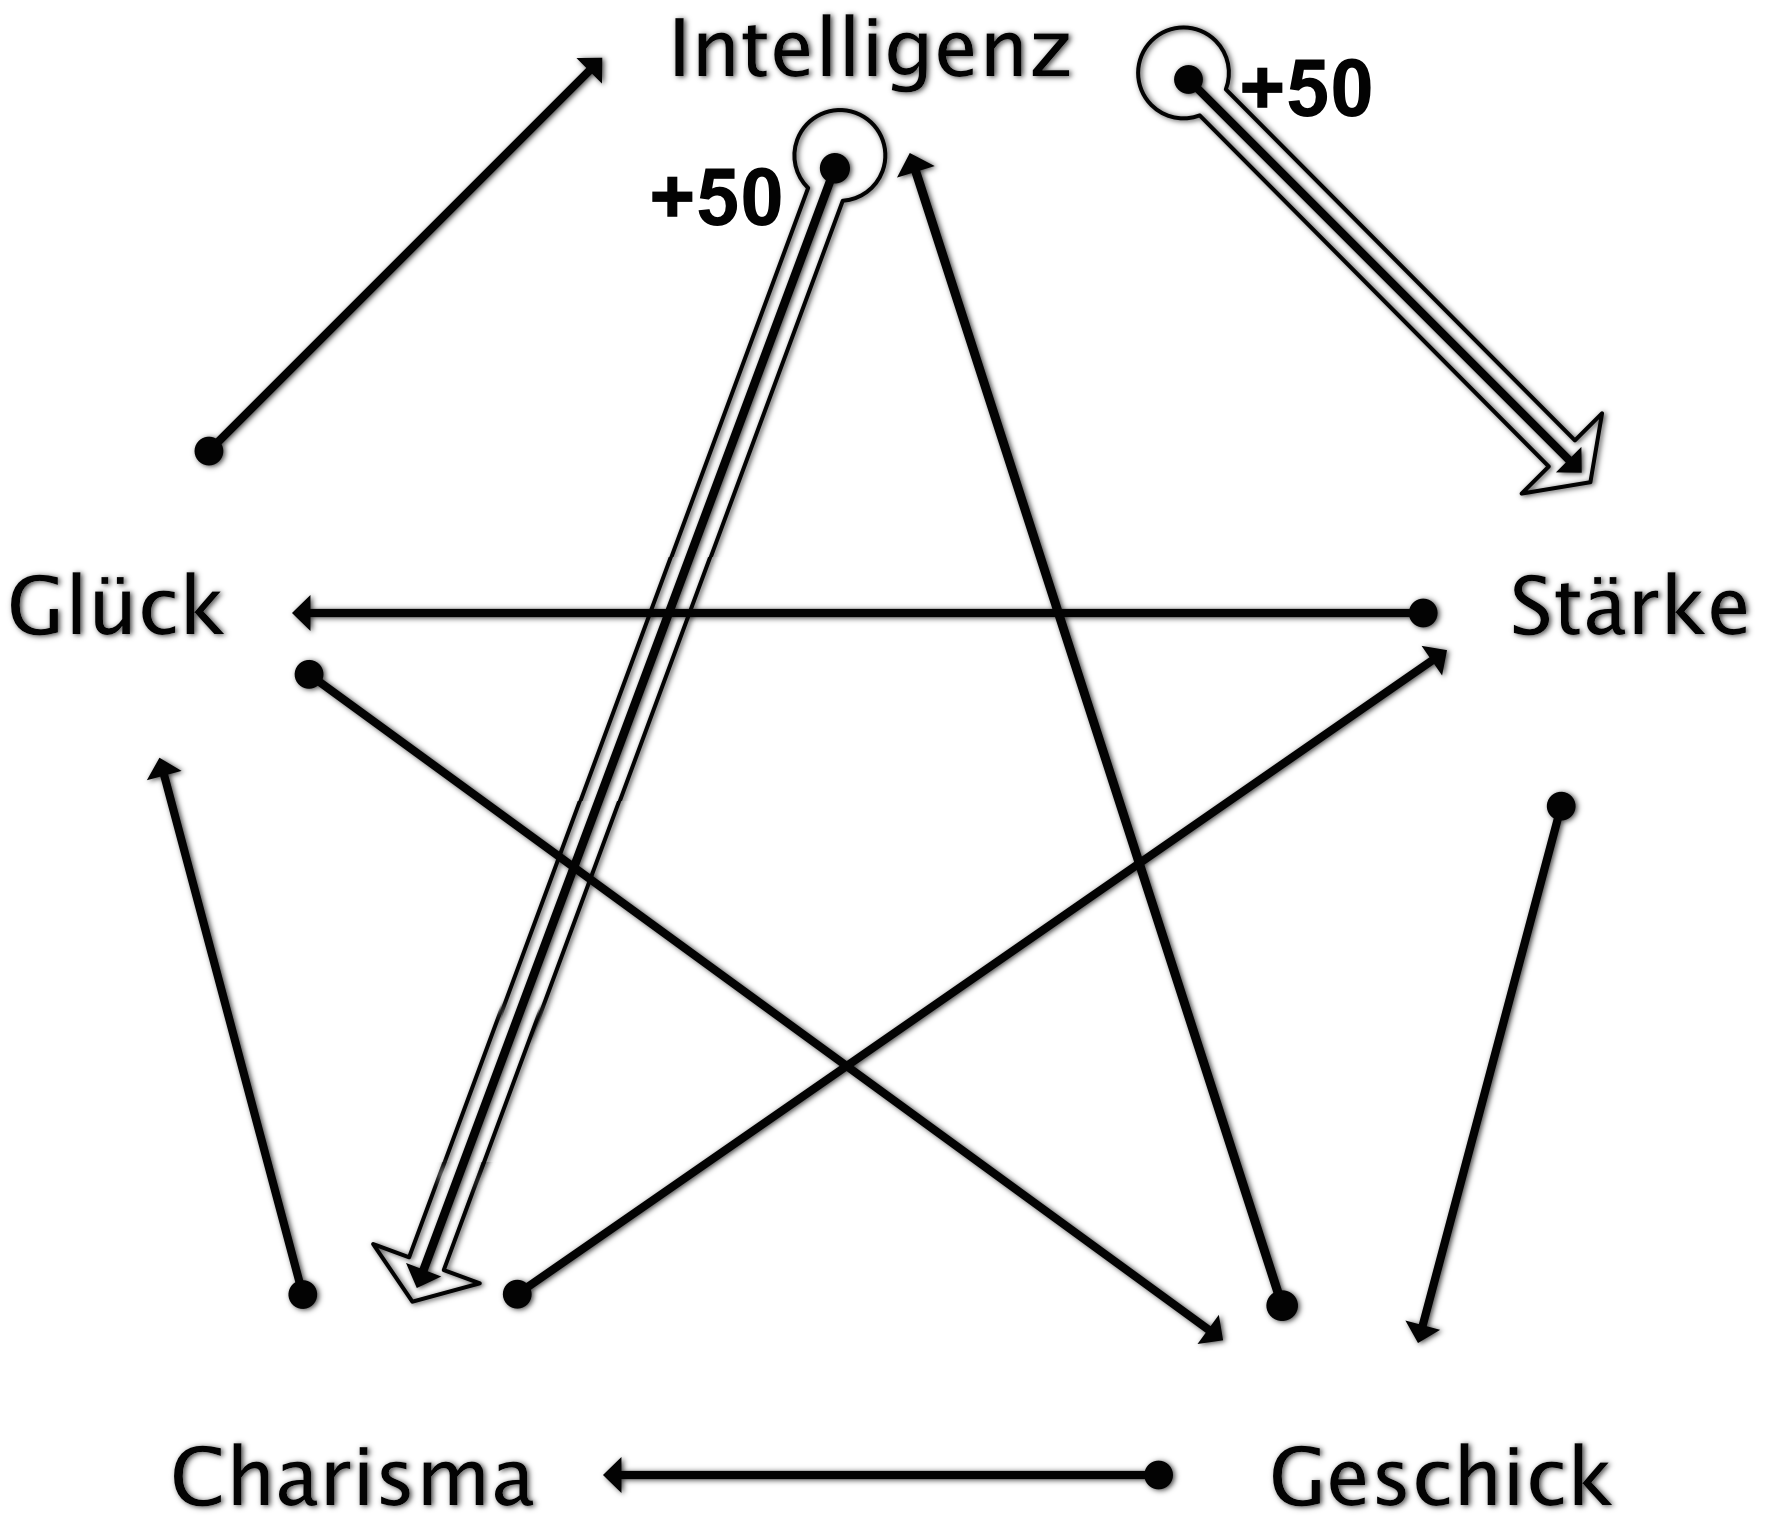
\includegraphics[width=.6\textwidth]{files/as/skillsPlus}
    \caption{Kampfsystem im Spiel. Die Pfeilspitzen zeigen auf das unterlegene Attribut. Das schlagende Attribut erhält +50 Punkte}
    \label{pic:ASSkills}
\end{figure}
     
Den einzelnen Attributen ist ein Wert zugeordnet. Beim Fangen eines Tieres, werden die Werte zufällig zwischen 1 und 100 für jedes einzelne Attribut festgelegt. Je höher ein Wert ist, desto mächtiger sein zugehöriges Attribut. Durch die zufällig festgelegten Werte werden die Attribute nicht mehr direkt geschlagen. \\
Ist bei einem \textbf{Kampf} ein Attribut im Vorteil (Intelligenz schlägt Stärke und Charisma), wird sein zugehöriger Wert für diesen Kampf um 50 Punkte erhöht (Intelligenz erhält 50 zusätzliche Punkte). Ein Intelligenzwert von 20 kann so beispielsweise einen Stärkewert von 71 nicht mehr schlagen. \\
Nachdem das Tier auf dem Smartphonebildschirm angezeigt wurde, wird der Spieler dazu aufgefordert für das Tier ein \textbf{Revier} anzulegen.  Das Revier kann an einem beliebigen Ort eingerichtet werden und hat einen Durchmesser von einhundert Metern. Das Revier ist ein Gebiet, das das Tier bewacht. Mit dem Anlegen des Reviers muss gleichzeitig ein Attribut auswählt werden. Das Tier verteidigt ab diesem Zeitpunkt sein Revier mit dem gewählten Attribut. Wird das bewachte Gebiet von einem anderen Mitspieler betreten, wird ein Kampf zwischen beiden beteiligten Tieren ausgelöst. Der Angreifer wählt ein Attribut für sein Tier, dies wird mit dem Attribut des verteidigenden Tiers verglichen und der Sieger wird bestimmt. Dieselben Spieler können nur einmal pro Tag gegeneinander kämpfen. Gewinnt ein Spieler einen Kampf, erhält er Punkte für seinen Sieg. Der Verlierer erhält keine Punkte. Die erhaltenen Punkte werden als \glqq Victory Points\grqq\, kurz VP, bezeichnet. \glqq Victory Points\grqq\ sind die Basis für das \textbf{Highscore System}. Neben den Punkten, die durch Siege errungen werden, erhält ein Spieler zusätzlich Punkte für jede Minute der Lebenszeit seines Tieres. Die Lebenszeit ist auf fünf Tage begrenzt und entspricht einem Spielzyklus. \\


Bei der allgemeinen Beschreibung handelt es sich um ein grundlegendes Spielkonzept, das durch verschiedene Module erweitert werden kann. Die Module sind: \\

\item[Spielzyklus] - 
Ein Spielzyklus ist auf fünf Tage festgelegt. Danach muss ein Spieler ein neues Tier fangen, da er nicht gleichzeitig mehrere Tiere besitzen kann. Der Spielzyklus muss in der weiteren Entwicklung angepasst werden. Er ist für die Basisversion kurz gewählt worden, um mehr Abwechslung in das Spiel zu bringen. Im Vorfeld kann aber nicht genau bestimmt werden, wie viel Zeit ein Spieler in der Regel mit einem bestimmten Tier spielen möchten. Es könnten auch dynamische Spielzyklen genutzt werden. Bei jeder Änderung muss darauf geachtet werden, das das Punktesystem dem Spielzyklus anzupassen.

%Balance
%Da Spieler vielleicht lieber mehr Zeit mit einem Tier verbringen möchten, bietet sich auch an die Spielzyklen dynamisch zu gestalten, so das ein Zyklus durch bestimmte Gegenstände verlängert werden kann. Die Punkte die ein Spieler erspielen kann stehen in Verbindung mit dem Spielsteht muss bei Änderungen stets auf das Punktesystem geachtet werden, damit es zu keinen großen Sprüngen bei den Punkten kommt.

\item[Karte] - 
Im Spiel steht dem Spieler eine Landkarte zur Verfügung. Besitzt ein Spieler noch kein Tier, werden fangbare Tiere in seiner Nähe angezeigt. Hat ein Spieler ein Tier gefangen, werden ihm Reviere angezeigt. So kann er über die Karte sein Revier anpassen oder eine Route planen, um das Revier eines anderen Spielers zu erreichen. 

\item[Fangvorgang] - 
Tiere werden auf der Karte angezeigt. Ein Spieler muss sich zu einem Tier hinbewegen. Der Bereich in dem ein Tier gefangen werden kann entspricht, der Reviergröße und hat auch einen Durchmesser von einhundert Metern. Der Prozess des Fangens kann im Laufe der Entwicklung des Spiels ausgebaut werden. Es könnten beispielsweise Köder im Spiel verwendet werden, die ein Spieler erwerben muss oder die durch Gesten mit dem Smartphone aktiviert werden. 

\item[Revier] - 
Jeder Spieler muss nach dem Erhalt eines Tieres erst ein Revier für sein Tier anlegen, damit er die volle Funktionalität des Spiels nutzen kann. Der Durchmesser des Reviers beträgt einhundert Meter. Um ein Revier zu erstellen, muss der Spieler zusätzlich ein Attribut auswählen, mit dem sein Tier dieses Revier verteidigt. Dieses Attribut kann im Nachhinein jeder Zeit geändert werden. So wird ein Kampf in einem Revier nicht vorhersehbar. Reviere können während der Entwicklung des Spiels so erweitert werden, dass die Spieler eine Möglichkeit haben sie zu personalisieren. So kann ein Revier einen bestimmten Typ haben. Eine Bibliothek könnte so beispielsweise die Intelligenz des Verteidigenden Tieres steigern.

\item[Kampf] - 
Das Kampfsystem besteht aus fünf Attributen und den zugehörigen Werten. Diese Werte sorgen dafür, dass ein Kampf nicht immer nach dem gleichen Schema abläuft, da auch unterlegene Attribute gewinnen können. Durch die unterschiedlichen Werte wird zusätzlich einem Unentschieden vorgebeugt. Sollten dennoch das Attribut, und dessen Wert in einem Kampf bei beiden Spielern gleich sein, gewinnt der Spieler mit dem älteren Tier. Das Alter ist vom Zeitpunkt des Fangens anhängig. Das Kampfsystem bietet mit den fünf Attributen und den zugehörigen Werten nicht viel Tiefgang. Dieses Grundsystem lässt sich aber durch neue Elemente stark erweitern. So könnte ein Kampf beispielsweise über mehrere Runden andauern, eine Gestensteuerung zur Auswahl der Attribute entwickelt werden und Umgebungsdetails oder Gegenstände mit in den Kampf einbezogen werden.

\item[Attribut] - 
Ein Tier besitzt fünf Attribute. Diese werden beim Fangen des Tieres zufällig im Bereich zwischen 1 und 100 gesetzt. Um dem Spieler ein besseres Feedback zu geben beeinflussen die Attribute die Farbe der Tiere. Daher werden einem Spieler die Werte nicht ab Beginn des Spiels angezeigt. Erfahrene Spieler haben so die Möglichkeit die Werte eines Tiers einzuschätzen. Die Tage eines Spielzyklus entsprechen der Anzahl der Attribute. So wird jeden Tag der Wert eines anderen Attributes eingeblendet, damit neue Spieler ihren Wissensstand erweitern können. Im Laufe der Entwicklung könnten dem Tier neue Attribute hinzugefügt werden. So könnten beispielsweise Lebenspunkte eingeführt werden, die einen direkten Einfluss auf das Kampfsystem haben würden.


\item[Item] - 
In der Basisversion des Spiels sind noch keine Gegenstände vorhanden. Sie könnten aber Einfluss auf alle Elemente des Spiels haben. Die einzelnen Tiere und ihre Reviere könnten durch sie personalisiert werden. Sie könnten aber auch einen direkten Einfluss auf das Spielgeschehen haben, indem sie die Werte bestimmter Attribute beeinflussen. 


\item[Highscore System] - 
Für jede Minute die ein Tier am Leben ist, erhält ein Spieler sog. \glqq Victory Points\grqq\ . Das heißt in einem Standardspielzyklus von fünf Tagen erhält er mindestens 7200 Punkte. Besucht ein Spieler während eines Spielzyklus die Reviere der Tiere von anderen Spielern, kann er durch Kämpfe weitere Punkte erhalten. Der erste Sieg des Tages bringt einem Spieler 1440 VP, der zweite Sieg 1320 VP und der dritte Sieg 800 VP. Für jeden weiteren Sieg erhält ein Spieler nur noch 100 VP. Der erste Sieg ist genau so viel wert wie ein Tag im Leben eines Tieres. Durch diese Staffelung sollen Spieler dazu animiert werden täglich mindestens drei Siege zu erringen. Zusätzlich kann durch diese Stafflung erkannt werden, wie viel Zeit ein Spieler in das Spiel investiert. Die Punkte, die sich erspielen lassen, könnten in einer späteren Version des Spiels als Währung genutzt werden. So könnte ein Spieler beispielsweise Gegenstände erwerben, indem er sie gegen \glqq Victory Points\grqq\ eintauscht. 

\item[Story] - 
Von Beginn an war eine Hintergrundgeschichte für das Spiel geplant. Diese wird zum Spielen der ersten Versionen nicht benötigt. Sie sollte aber in einem späteren Entwicklungszyklus eingebaut werden. Denkbar wäre eine episodenbasierte Geschichte, so dass die Spieler in bestimmten Zeiträumen immer wieder neue Teile der Geschichte erleben können. 

%Um auf dem höchsten Niveau mitspielen zu können, muss so der Spieler mindestens drei Siege pro Tag erzielen.


%Ein Sieg bringt einem Spieler 10 VP. Zusätzlich gibt es für die ersten drei Siege täglich Bonus Punkte. Für den ersten Sieg erhält er 1430+10 VP, für den zweiten Sieg 1310+10 VP, für den dritten 790+10 VP und für alle weitern Siege danach wieder nur 10 VP. Durch diese Staffelung lässt sich beim Highscore deutlich erkennen welche Spieler viel und welche Spieler weniger gespielt haben. 


%1440, 1432, 1376, 1224, 440
%\begin{center}
%\begin{tikzpicture}
%
%\begin{axis}[domain=0:8,
%    samples=20,
%    xmin=0,   xmax=6,
%    ymin=0,   ymax=1500,
%    grid=both, no markers
%  ]
%\addplot +[thick] {(-8*(x^3))+1440};
%\end{axis}
%\end{tikzpicture}
%\end{center}


%\begin{center}
%\begin{tikzpicture}
%
%\begin{axis}[domain=0:8,
%    samples=40,
%    xmin=1,   xmax=3,
%    ymin=0,   ymax=1500,
%    grid=both, no markers
%  ]
%\addplot +[thick] {(-8*(x^4))+1438};
%
%
%
%\end{axis}
%
%
%\end{tikzpicture}
%\end{center}


%
%Highscore System
%5 Tage zeit
%
%1 Punkt = 1 Minute
%
%
%
%Tiere fangen
%    Farbe Nach Fähigkeit, Zeit, Ort 
%
%Tieren Revier zuweisen
%  %  Tier hat ein Revier im Umkreis von 50m 
%    Nur ein Revier pro Tier 
%  %  Wert wählen, mit dem ein Tier sein Revier verteidigt, 
%        kann im Nachhinein vom spieler geändert werden
%    
%    
%Tiere kämpfen lassen
%%    die selben spieler können nur einmal pro tag gegeneinander kämpfen
%%    Die Basis das Kampfsystems besteht auf einer erweiterten Version des alt bekannten Spiels, Schere, Stein, Papier und wird um 2 weiter Punkte erweitert. Die neuen Werte sind Stärke, Intelligenz, Geschicklichkeit, Charisma, Glück.
%
%%Die Abbildung \ref{pic:ASSkills} zeigt, wie die Werte gegeneinander aufgestellt sind. Somit schlägt zum Beispiel Intelligenz Stärke aber würde jedoch von Geschick selber geschlagen. Zu diesem recht einfachen Prinzip kommt aber noch ein Werte-System hinzu. Beim Fangen eines Tieres, werden die Werte zufällig zwischen 1 und 100 für jedes einzelne Attribut gewählt. 
%        %Auf dem Server befindet sich zudem eine Tabelle, die für bestimmte     Tiere bonus werte erhält. So kann man im weiteren Verlauf Gebiete definieren in denen beim Fangen ein Bonuswert von zum Beispiel 10 oder mehr Punkten gewährt wird.
%
%
%
%
%Karte 
%    Zeigt Reviere
%    Gegenstände 
%    Tiere
%
%
%%Die neue Grundidee des Spiels ist es verschiedene nach wie vor verschiedene Tiere zu fangen, jedoch ist die Lebensdauer eines Tiers stark beschränkt. Die Hauptresource die dem Spieler zur Verfügung steht ist Zeit. Dies soll dazu beitragen, das die Spieler sich genau überlegen wie sie mit der Zeit umgehen wollen. Durch die neuen Items, wird dieser Aspekt noch weiter gestärkt, denn keines der Items soll nur Vorteile bringen. Somit muss sich der Spieler bei jedem Gegenstand genau überlegen, ob er es wirklich einsetzen möchte. Dies ist ein ganz wichtiger Punkt. Denn jede Entscheidung des Spielers soll einen großen Einfluss auf das gesamte Spielgeschehen haben. Somit besteht die Hauptaufgabe darin, mit seinem Tier in 7 Tagen möglichst viele Punkte, die im weiteren Verlauf auch Victory Points genannt werden oder mit VP abgekürzt werden, zu sammeln. Diese kann der Spieler durch gewonnen Kämpfe erhalten oder jeweils einen für jede Minute, die sein Tier am Leben ist. 
%%Das fangen der Tiere gestaltet sich so, dass dem Spieler einfach durch drücken des Tier aufspüren Knopfes ein neues Tier generiert wird. Dieser Vorgang lässt sich natürlich noch weiter ausschmücken, indem man vielleicht ein kleines minispiel hinzufügt, mit dem man das tier an sich gewöhnen muss. Das gefangene Tier unterscheidet sich je nach Standort. so wird die Farbe je nach Tageszeit und Ort. 
%%Hat mein ein tier gefangen, wird man dazu aufgefordert ein Revier für sein tier zu markieren. Reviere sind die gebiete, in denen die Tiere "außerhalb" des telefons leben. Es ist so zu verstehen, das ein Tier in einem Revier verweilt und mittels des Spiels eine Verbindung dazu hergestellt wird. Außerdem sind Reviere interaktive Gebiete. Ein Spieler kann jedoch nur ein Revier selber erstellen. Er kann aber mehrere Reviere erspielen, indem er andere Spieler besiegt und deren Reviere für sich beansprucht. Des weiteren werden alle Reviere in der aktuellen Umgebung des Spielers auf der Karte im Spiel angezeigt. Somit kann ein Spieler sich auf der Karte ein Revier aussuchen, sich dorthin begeben und dieses nach einem erfolgreichen Kampf für sich beanspruchen. Zum markieren des Reviers gehört zudem einen Wert des eigenen Tieres auszuwählen, mit dem es Kämpft. Daher wird nun erst etwas genauer auf das Kampfsystem eingegangen. Die Basis das Kampfsystems besteht auf einer erweiterten Version des alt bekannten Spiels, Schere, Stein, Papier und wird um 2 weiter Punkte erweitert. Die neuen Werte sind Stärke, Intelligenz, Geschicklichkeit, Charisma, Glück.
%
%
%
%
%
%%Somit könnte Tier A so aussehen:
%%
%%Stärke    Intelligenz    Geschick    Charisma    Glück
%%44        65             74          89          12
%%
%%Und Tier B so:
%%Stärke    Intelligenz    Geschick    Charisma    Glück
%%55        94             70          61          49
%
%
%%Durch die Werte bei den Attributen wird nun nicht mehr direkt geschlagen, sondern ein Bonus verteilt. Würde wie in der Abbildung Monster A Monster B mit dem Stärke Attribut angreifen, und der Besitzer von Monster B Geschick als Attribut wählen, würde Monster A einen Bonus von 50 Punkten auf sein Attribut erhalten und somit Monster B besiegen. Nach dem Sieg werden die Victory Points vergeben. Der Besitzer von Monster A erhält nun entsprechend der Anzahl an Spielen, die er am aktuellen Tag getätigt hat.
%Die lässt sich am folgenden Graphen zeigen:
%
%\textbf{Victory Points:}
%
%
%
%Die Formel für die VP lässt sich so berechnen: $(-8*(x^3))+1440$. 
%Daraus ergibt sich, dass der erste Sieg an einem Tag 1044 VP dem Spieler einbringt. Für einen weiteren Sieg würde er nur noch 1432 Punkte erhalten. Dies läuft solange weiter, bis man nach dem fünften Sieg nur noch 440 Punkte erhält. Ein sechster Sieg würde weiterhin 440 Punkte bringen. Dies hat zur Folge, dass Spieler die sehr viel Spielen nicht viel mehr Punkte bekommen, als Spieler die am Tag nur 2-3 Runden Spielen können. Es gibt aber weiterhin so viele Punkte das es sich auch lohnt weitere Runden zu spielen um einen höheren Highscore zu erreichen. 
%
%1440, 1432, 1376, 1224, 440
%
%Ziel des Spiels ist es einen möglichst hohen Highscore zu erreichen, dadurch können die Spieler auf einer Liste vergleichen, wie gut sich im Gegensatz zu anderen Spielern abschneiden. Der Highscore setzt sich zusammen aus der Lebenszeit, die das Tier überlebt hat und den victory points, welche der spieler durch das erzielen von siegen erhält. Dies geschieht durch eine einfache Addition, Lebenszeit (in Minuten) + Victory Points).
%Um den Highscore leichter lesbar als in vielen anderen Spielen zu machen wird die Lebenszeit in Minuten gemessen, was auch den Vorteil bringt, das sie zeitkritisch ist, aber trotzdem relativ genau ist.
%Der maximale Puntkestand, den man ohne Kämpfe erreichen kann ist daher MaxLebenszeit: (7*24*60 = 10080) und ist die Anzahl der Minuten, die eine Woche hat. 
%Dies soll auch als Referenzwert dienen, da man ihn leicht überschreiten kann aber auch durch einige Fehlentscheidungen auch unterschreiten kann.
%
%Um die Kämpfe und den gesamten Spielablauf spannender zu gestalten, kann Spieler Items einzusetzen. 
%Die folgende Tablle zeigt, welche Items welchen Bonus bringen.
%Stärke – Strength:		Hantel\\
%Intelligenz – Intelligence: 		Buch\\
%Geschicklichkeit – Dexterity:	Werkzeug\\
%Charisma – Charisma:		Spiegel\\
%Glück – Luck:				Kleeblatt \\
%Obwohl diese standard Items, von Begin für den Spieler verfügbar sind, können sie jedoch nicht beliebig eingesetzt werden. Wird ein Gegenstand eingesetzt, muss der Spieler einen Tag der Lebenszeit seines Tieres dafür bezahlen. Zudem können die Gegenstände auch nicht beliebig oft eingesetzt werden. Benutzt man das erste mal einen Gegenstand, erhält das Tier +50 Punkte auf den gewünschten wert. Wird ein zweites Item eingesetzt, werden nur noch 25 Punkte gutgeschrieben. Die Punkte werden so lange reduziert, bis ein Item nur noch 7 Punkte auf den jeweiligen Wert addiert. Die Punkte werden also in jedem Schritt halbiert und danach aufgerundet. 
%Items: +50,  +25, +13, +7
%
%Die Kämpfe laufen wie folgt ab. Nachdem ein Spieler das Revier von einem anderen Spieler bzw. Tieres betritt während das Spiel auf dem Telefon läuft, kann er einen der oben genannten Werte auswählen, wie z.B. Stärke oder Intelligenz. Mit diesem Wert wird dann das andere Tier in seinem Revier angegriffen und verteidigt sich mit dem Wert, den der andere Spieler zuvor gewählt hat. Sollte es nach Berechnung des Bonus trotzdem zu einem Unentschieden kommen, gewinnt das Tier, das älter ist. Dies bedeutet, das es so gut wie gar nicht zu einem Unentschieden kommen kann, da nicht nur die Werte identisch sein müssten, sondern auch die Sekunde, in der beide Tiere gefangen wurden. Zudem soll es nicht möglich sein ein Revier mehrmals an einem Tag zu betreten. Dadurch soll verhindert werden, dass ein Spieler, nachdem er herausgefunden hat, mit welchem Wert er am besten antritt, dies andauernd wiederholt um schnell viele Punkte zu erreichen. Dies hat zudem den Vorteil, das die Spieler sich weiter bewegen müssen um Kämpfe zu bestreiten. Des Weiteren werden auch trotz einer Niederlage keine Punkte abgezogen. 
%
%Um das Kampfgeschehen nicht zu stark vorhersehbar zu machen, werden dem Spieler die Werte des eigenen Tieres nicht angezeigt. Sondern erst nach und nach zufällig aufgedeckt. Es wird jeden Tag ein neuer Wert angezeigt. Somit erhält der Spieler jeden Tag eine Information mehr über sein Tier.
\end{description}
%\section{Aktualisierte Anforderungen}
%\label{cha:ext_server}
%Im folgenden Kaptiel wird auf die Anforderungen eingegangen, die aus Sicht des Autors nötig sind, um das Spiel umzusetzen.
%
%GUI mit verschiedenen Fenstern, bzw. Layern
%folgende Informationen sollen einsehbar und Funktionen Nutzbar sein.
%
%Tier: idle screen
%Der Hauptbildschirm, sowie die Anzeige während der Spieler inaktiv ist unterteilt sich in 2 unterschiedliche Modi. Sollte der Spieler, wie es zu Spielbeginn vorgesehen ist, schon ein Tier haben, wird es auf diesem Bildschirm angezeigt. Es können verschiedene Animationsketten durchlaufen werden und die Hintergrundmusik wird abgespielt. Sollte die erste Spielphase abgelaufen sein, wird ein Knopf angezeigt, mit dem man ein neues Tier "erstellen" kann. Nach Betätigung des Knopfes werden die Werte für das neue Tier automatisch anhand der Datenbank auf dem Server generiert und es werden wieder die Animationsketten, des Tieres wiedergegeben. 
%
%items: overlay
%Über einen Knopf am unteren Rand des Bildschirms gelangt man zu den Gegenständen, die ein Spieler einsetzen kann. Nach Betätigung wird ein Overlay Menü angezeigt, auf dem der Spieler die entsprechenden Items, die er einsetzten kann angezeigt werden, zudem wird ein kleiner Infotext daneben angezeigt, der genauere Informationen darüber gibt, welchen Einfluss das nebenstehende Item hat. Des Weiteren befindet sich am Gegenstand in der rechten unteren Ecke eine Zahl, die angibt, wie oft man den Gegenstand noch benutzen kann.
%
%status: overlay
%Im Status Fenster wird angezeigt, an welcher Position man sein Tier gefangen bzw. generiert hat. Zudem sind hier Informationen über das Alter des Tieres zu finden. Damit der Spieler sehen kann, wie lange sein Tier schon lebt und wie viel Lebenszeit ihm noch zur Verfügung steht. Hinzu kommen, die einzelnen Werte des Tieres, also Stärke, Intelligenz, Glück, Charisma, Geschick. Bei diesen Werten ist jedoch zu beachten, dass sie nicht von Anfang an in Gänze angezeigt werden, sondern jeden Tag ein zufälliger Wert aufgedeckt wird.
%
%options: overlay
%Die Optionen sind ein weiteres Fenster, das über den Idle Screen gelegt wird. Hier kann eingestellt werden, ich welchem Intervall die Position des Spielers abgefragt, wird. Hierzu hat der Spieler einen Schieberegler, mit dem er das Intervall in einem Zeitraum von 10 Sekunden und 5 Minuten eingestellt werden kann. Zudem gibt es eine Checkbox, in der gewählt werden kann, ob jeweils beim starten der App sofort die Position bestimmt werden soll. Weitere Optionen sind zum einen die Lautstärke der Hintergrundmusik sowie die Lautstärke der Soundeffekte, die bei dem betätigen eines Buttons abgespielt werden. Zum anderen eine weitere Checkbox, mit der der Spieler entscheiden kann, ob er auch außerhalb der App darüber benachrichtigt werden möchte, wenn ein anderer Spieler sich in einem Kampf mit ihm befindet.
%
%karte: map screen
%Der Karten Bildschirm teilt sich in drei Anzeigepunkte auf. Durch einen Reiter am rechten Bildschirmrand kann der Spieler wählen welchen Teil er sehen möchte. Der obere Reiter ist mit dem Namen Umgebung betitelt und Zeigt an, welche Reviere sich in direkter Umgebung des Spielers befinden. Dabei werden nur Reviere berücksichtigt, die der Spieler am aktuellen Tag noch nicht besucht hat. Seine eigenen Reviere werden dort auch nicht angezeigt. Es werden also nur Orte dargestellt, an denen der Spieler spielen kann. Der mittlere Reiter trägt den Titel besucht. Hier werden Reviere angezeigt, in denen der Spieler am aktuellen Tag gekämpft hat. Der untere und somit letzte Reiter ist mit dem Titel Reviere betitelt. Hier kann der Spieler sehen, welche Reviere er für sich beansprucht hat. 
%
%kampf: battle screen
%Der Kampfbildschirm wird automatisch angezeigt, sobald ermittelt worden ist, das sich der Spieler im Revier eines anderen Spielers befindet. Der Spieler, der das Revier eines anderen Spielers betritt, erhält aus seinem Smartphonebildschirm ein neues Fenster auf dem er das Tiere des konkurrierenden Spielers sehen kann. Sternförmig um das Tier des Gegners werden die Werte angezeigt mit denen er angreifen kann. Nachdem er seine Wahl getroffen hat, erhält er noch eine kurze Einblendung, die ihn über Sieg oder Niederlage benachrichtigt.
%
%Highscore
%Der letzte Bildschirm zeigt die Rangliste der Spieler an. Es handelt sich hierbei lediglich um eine Liste, auf der der Spieler sehen kann, auf welcher Position er sich aktuell befindet. 

%\section{Umgang mit Problemstellungen} 
%%\label{sec:}
%
%
%\subsection{Gefahrenzonen} 
%%\label{sec:}
%Es gibt mehrere verschiedene Möglichkeiten Gefahrenzonen auszuschließen. Der erste Gedanke könnte hierbei sein, die Gebiete zu sperren. Dies könnte geschehen, indem sich der oder die Entwickler Karten zur Hand nehmen und entscheiden, welche Gebiete Gefahrenzonen sind und diese zu markieren. Damit einher geht aber ein sehr großer Zeitaufwand. Da die Karten nicht nur ausgewertet werden müssen, sondern auch für die Spielclients festgehalten muss, an welchen Orten das Spiel gespielt werden kann. Hinzu kommt die Fehleranfälligkeit. Da die Karten wie gesagt ausgewertet werden müssen, sollte man so ein Projekt sogar nur einem Land wie zum Beispiel Deutschland ausführen, wäre es kaum möglich alle Gebiete vernünftig abzudecken. Ein anderer Ansatz solche Gebiete zu sperren, wäre einen Alogrihtmus zu entwicklen, welcher Karten analysieren kann. Doch hierzu muss erst einmal festgestellt werden, wo und in weit es sich um Gefahrenzone handelt. Somit ist dieser Ansatz auch eher unpraktikabel. Das einzige, was von Umfang her entwickelbar wäre, wäre ein System, bei dem die Spieler selber entscheiden können, ob ein Gebiet in die Kategorie Gefahrenzone fällt. So könnte man im Spielclient in den Optionen eine Funktion anbieten, die den aktuellen Ort als Gefahrenzone, dies könnte dann wiederrum von einem kleineren Team kontinuirlich bearbeitet werden und so in die Datenbank eingetragen werden. Zu guter letzt gibt es aber noch eine andere Möglichkeit, die allen vorhergegangenen Praktiken unnötig machen würde. Hierbei sollte versucht werden Gefahrenzonen für Spieler unatraktiv zu machen und dies schon im zugrundeliegenden Spielkonzept beinhalten. Die Frage die sich dahinter verbirgt, ist die Frage, wie erreiche ich es Spielern leicht zugängliche Orte schmackhaft zu machen. Beim geocaching verhält es sich genau gegenteilig. Denn der Schwierigkeitsgrad beim Geochaching steigt mit der Zugäglichkeit des Caches. Ein spieler der einen Cache gehoben hat, welcher sich mitten unter einer Brücke befindet musste viel mehr auf sich nehmen als wenn er einen Cache gehoben hätte, welcher sich am Wegrand im Graben befindet. Durch die größere aufgewandte Arbeit, ist wie zuvor beschrieben auch das Glücksgefühl umso größer. Somit entsteht eine Spirale. Die Caches werden immer besser und unzugänglicher versteckt und die Spieler setzen immer mehr Werkzeuge ein um diese zu erreichen. In einem Videospiel hat man jedoch den Vorteil, das man den Schwierigkeitsgrad an vielen anderen Stellen anpassen kann. Nimmt man jetzt die Reviere in Augenschein, die die Spieler in dem zu entwickelnden Spiel erstellen sollen können, so muss darauf geachtet werden, dass die Zugänglichkeit der Ort dieser Reviere nur bedingt beeinflusst. Dadurch das der Spieler pro Tag diese Reviere aufsuchen sollte und auch Spieler dessen Reviere besucht werden Boni erhalten, würde somit die Spieler eher anspornen häufig besuchte und leicht erreichbare Orte als Revier zu markieren. Als Bonus könnte man zusätzlich noch die Funktion einbauen, dass Reviere markiert werden können, sollte ein verstoß oder ein Gefahrengebiet vorliegen. 
\section{Evaluation der neuen Spielidee} 
\label{Abschnitt:EvaNeu}
Die neue Spielidee ist anhand der in Abschnitt \ref{Abschnitt:AttUXEva} vorgestellten Evaluation ausgewertet worden. Für diese Evaluation wurde ein sog. \glqq Pen and Paper\grqq\ Prototyp angefertigt. Dazu wurden mehrere Tiere auf Spielkarten gedruckt. Zwei Beispiele dafür sind in Abbildung \ref{pic:pnpPrototyp} dargestellt. Diese wurden in einem Waldstück verteilt. \\
Die Revierbestimmung wurde bei diesem Test vernachlässigt und auch die Attribute der Tiere wurden jederzeit angezeigt. Sobald sich zwei Spieler mit ihren gefunden Tieren begegnet sind, konnte ein Kampf beginnen. 
\begin{figure}[H]
    \centering
    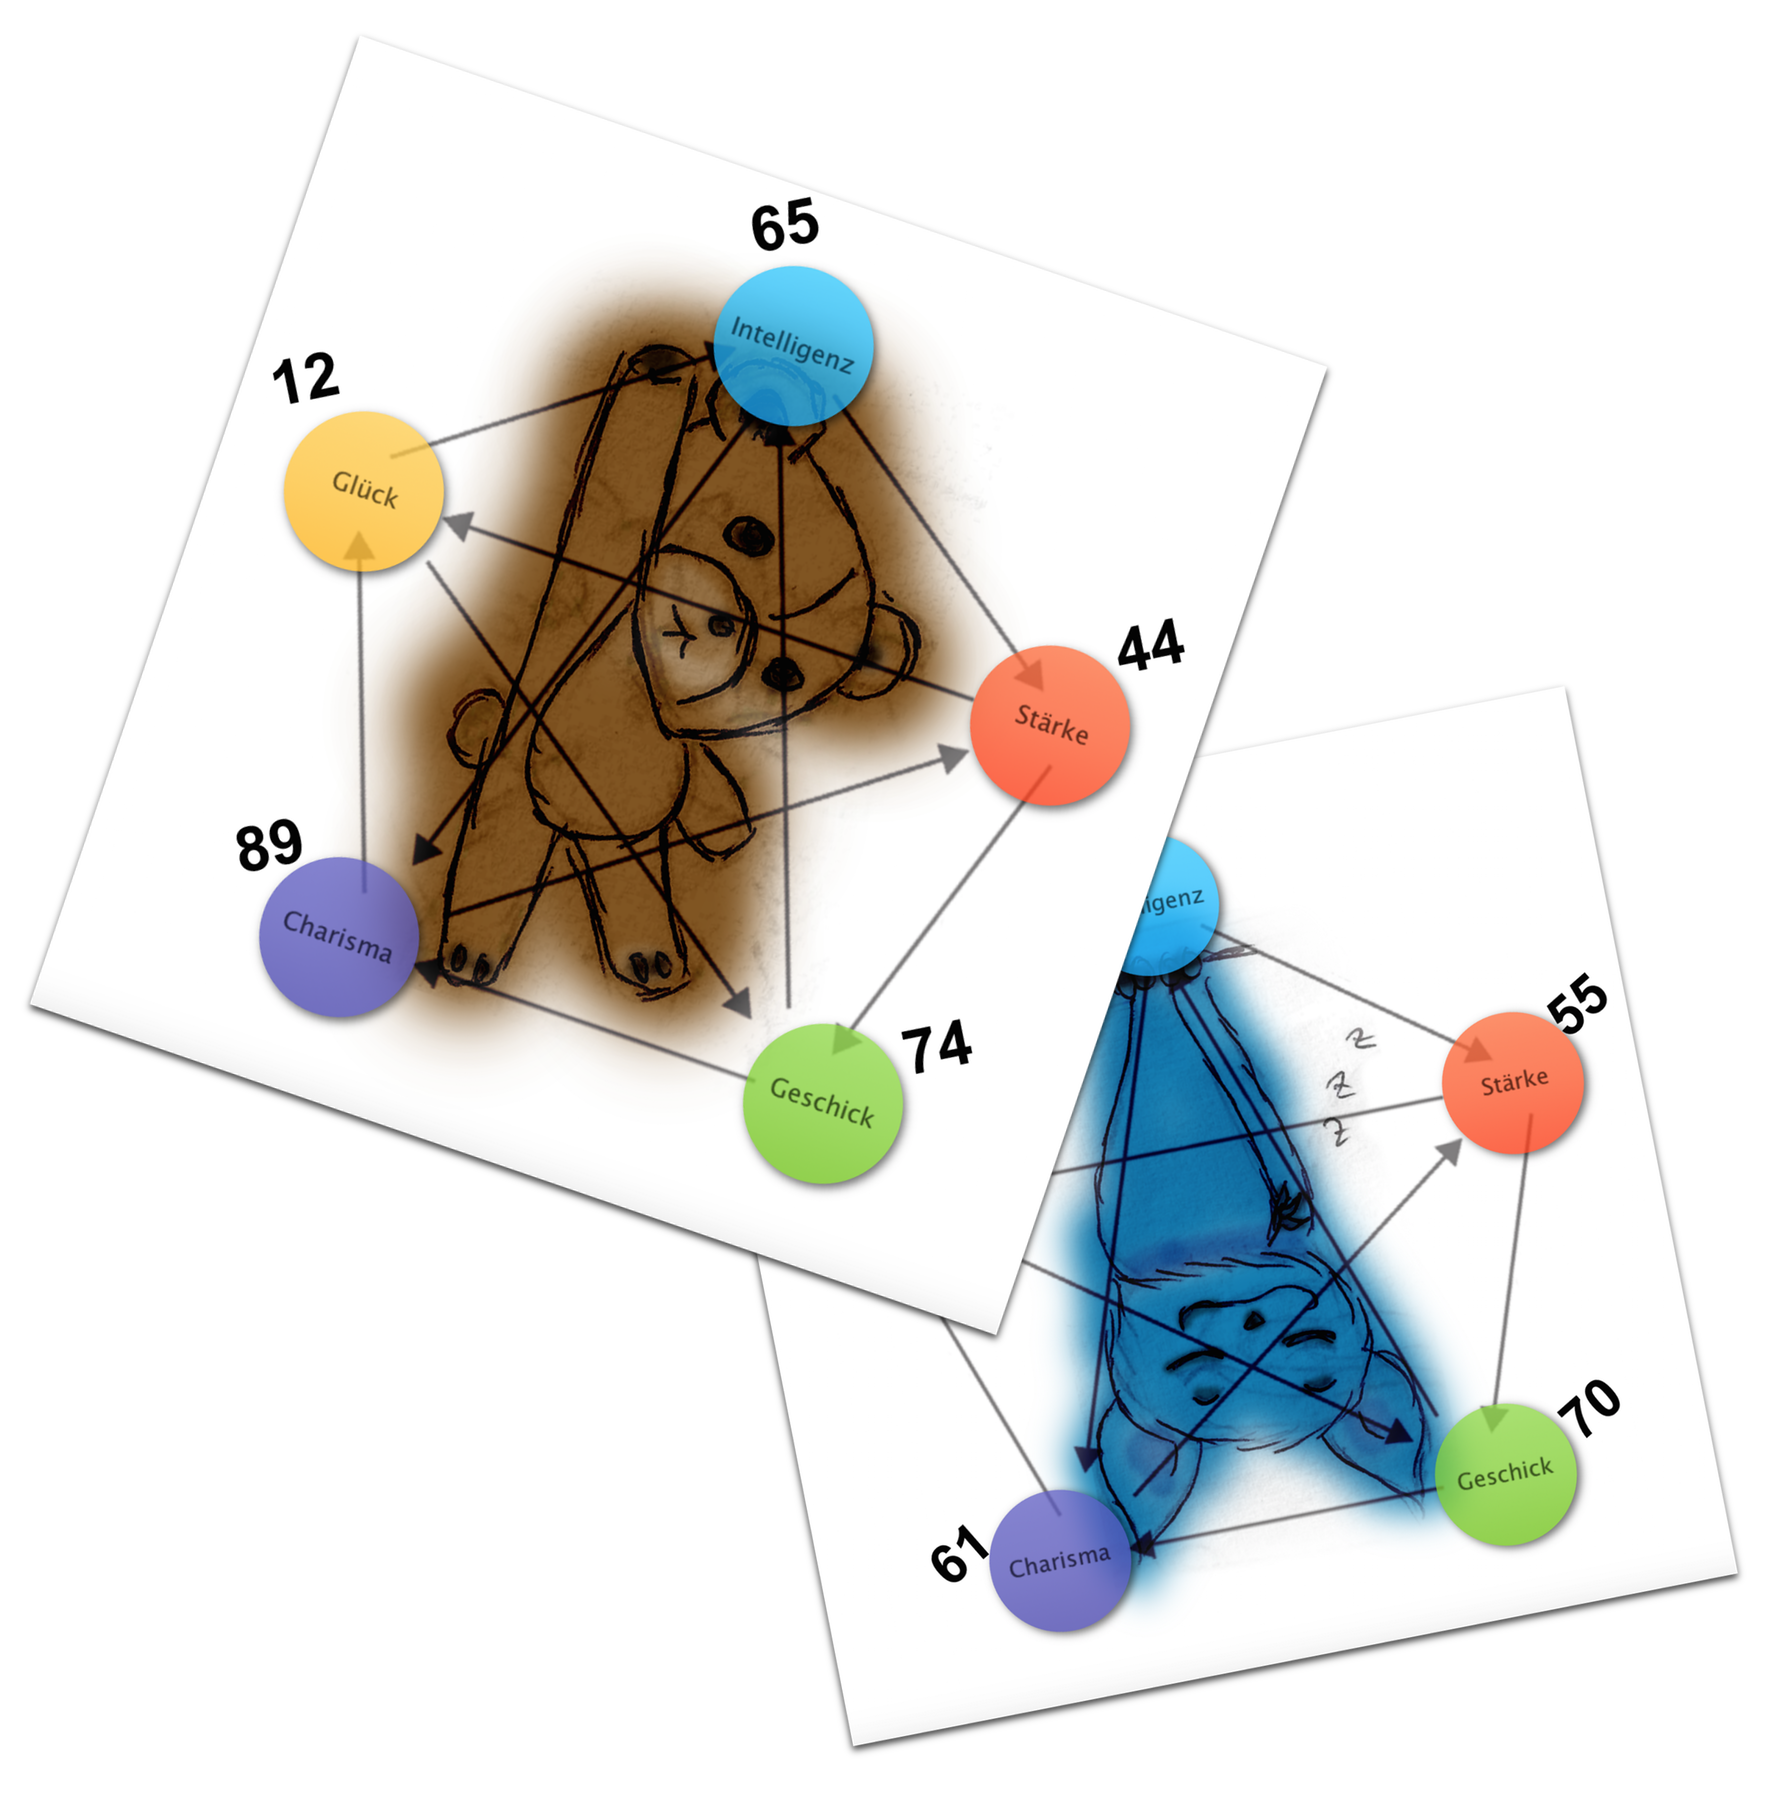
\includegraphics[width=0.8\textwidth]{files/feldtest}
    \caption{Pen and Paper Prototyp Spielkarten}
    \label{pic:pnpPrototyp}
\end{figure}
 




%Im Anschluss daran ist ein \glqq Pen and Paper\grqq\ Prototyp der neuen Spielidee entwickelt worden, der mit Hilfe eines abgewandelten AttrakDiff-Fragebogens nach Abschnitt \ref{Abschnitt:MethodenEvaluationUX} entwickelt worden ist.
Dieser Test wurde an einem Tag durchgeführt. 26 Personen haben daran teilgenommen. Im Anschluss an das Spiel wurde von jedem Spieler ein Evaluationsbogen ausgefüllt. Die Kriterien der User Experience, die ermittelt werden sollten sind Kaufentscheidung, Zugänglichkeit, Atmosphäre, Bedienung, Fortschritt, Tiefgang, Sozial Interaktion. In Abbildung \ref{pic:mySpecialUXEval} werden die mit den Kriterien verbundenen Antonyme mit der dazugehörigen Bewertung dargestellt. 



\begin{figure}[H]
    \centering
    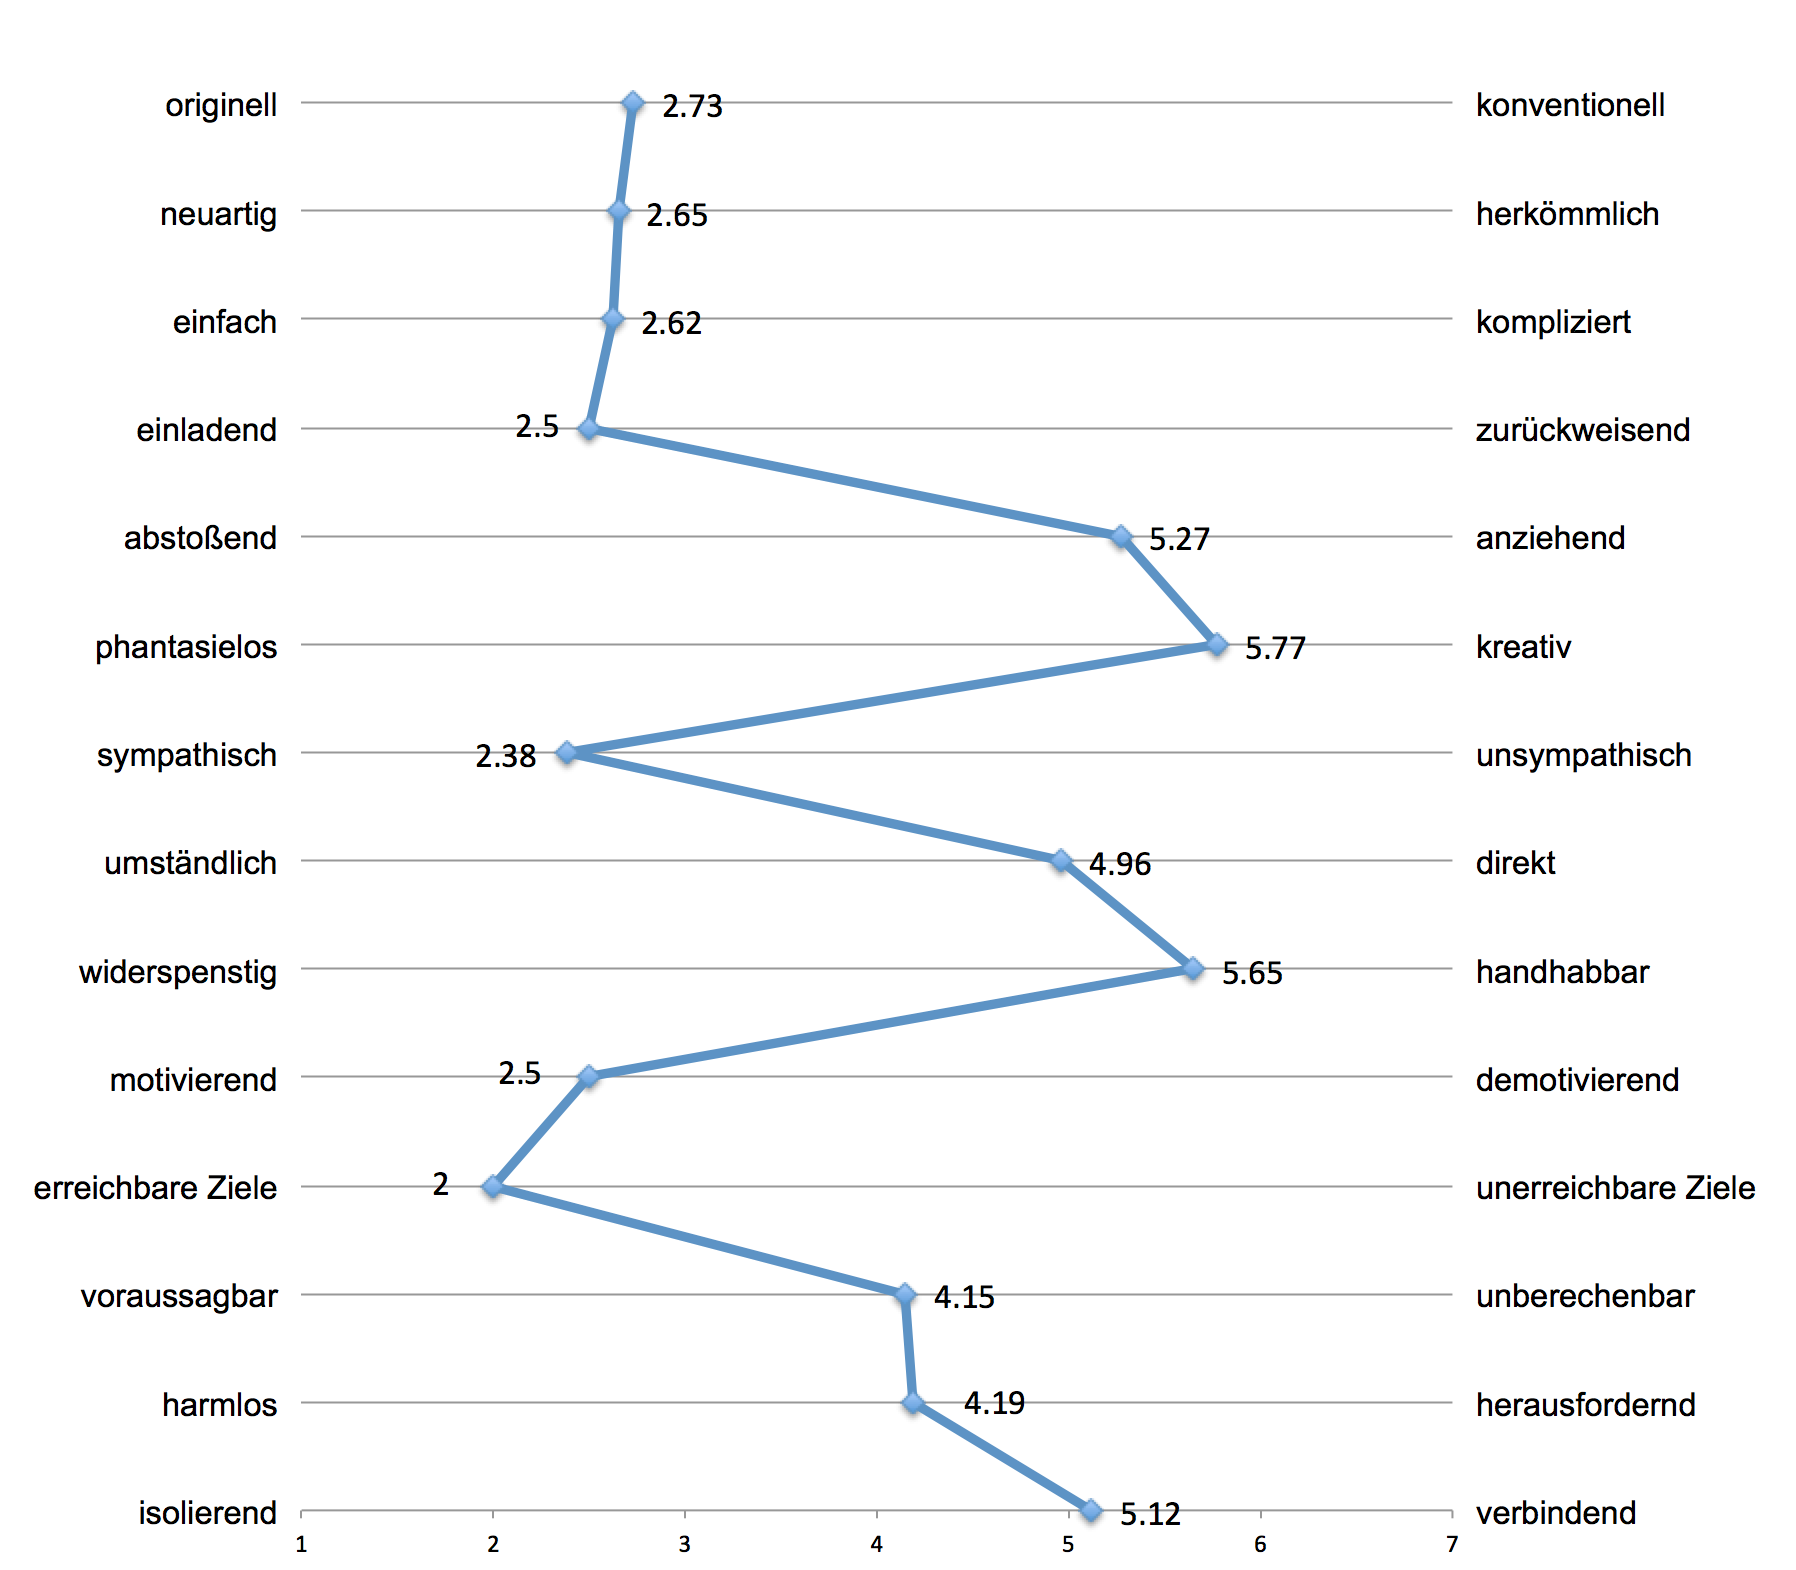
\includegraphics[width=1\textwidth]{files/statistik/umfrage2Ergebnisse}
    \caption{Ergebnis der User Experience Evaluation}
    \label{pic:mySpecialUXEval}
\end{figure}
 
Die Einschätzung der Antonyme konnte auf einer Skala von 1 bis 7 vorgenommen werden. 


\begin{description}
\item[Kaufentscheidung:]\
\begin{itemize}

\item Die grafische Präsentation wurde mit 2,73 als relativ originell empfunden. 

\item Das Spielkonzept wurde mit 2,65 als relativ neuartig empfunden. 


\end{itemize}
\item[Zugänglichkeit:] \ 
\begin{itemize}
\item Der Einstieg in das Spiel wurde mit 2,5 als relativ einladend empfunden.

\item Der anschließende Spielverlauf wurde mit 2,62 als relativ einfach empfunden.
\end{itemize}


\item[Atmosphäre:]\ 
\begin{itemize}

\item Die Ästhetik im Spiel wurde mit 5,27 als relativ anziehend empfunden.

\item Die Handlung im Spiel wurde mit 5,77 als relativ kreativ empfunden.


\item Die Charaktere im Spiel wurden mit 2,38 als relativ sympathisch empfunden.
\end{itemize}




\item[Bedienung:] Für den Pen and Paper Prototyp wurden nur die simpelsten Interaktionen mit den Spielkarten erwartet. Aber auch dieses Ergebnis steht vor dem Hintergrund, dass Æthershards in zukünftigen Versionen auf Smartphones gespielt werden kann.
\begin{itemize}



\item Die \glqq Menüs\grqq\ im Spiel wurden mit 4,96 als relativ direkt empfunden.


\item Die \glqq Steuerung\grqq\ im Spiel wurde mit 5,65 als relativ handhabbar empfunden.
\end{itemize}


\item[Fortschritt:] \ 
\begin{itemize}
\item Der Lernerfolg im Spiel wurde mit 2,5 als relativ motivierend empfunden.

\item Errungenschaften im Spiel wurde mit 2 als relativ erreichbare Ziele empfunden.

\end{itemize}


\item[Tiefgang:] \ 
\begin{itemize}
\item Der Schwierigkeitsgrad der Situationen des Spiel wurde von einigen Probanden als voraussagbar und von anderen als unberechenbar empfunden. Die gesamte Skala wurde abgedeckt. Es hat sich der Mittelwert von 4,15 ergeben.

\item Der Schwierigkeitsgrad der zu lösenden Aufgaben wurde von einigen Porbanden als relativ harmlos und von anderen als relativ herausfordernd angesehen. Die Skala von 2 bis 6 wurde abgedeckt. Es hat sich der Mittelwert von 4,19 ergeben.
\end{itemize}




\item[Soziale Interaktion:]\ 
\begin{itemize}

\item Das Spiel wurde mit 5,12 als relativ verbindend empfunden.

\end{itemize}




\end{description}


Die User Experience Evaluation zeigt, dass der Prototyp eine gute User Experience besitzt. Die Ergebnisse könnten teilweise durch den Pen and Paper Prototypen abgefälscht worden sein. Es würde sich anbieten den Prototyp so zu erweitern, das er auf einem Smartphone lauffähig ist. Dann könnte in einer weiteren Evaluation erneut die User Experience bestimmt werden. So könnten auch die Abweichung zwischen Softwareprototyp und Pen and Paper Prototyp bestimmt werden. 